\documentclass[.../main.tex]{subfiles}

\begin{document}

    This chapter continues to describe the proposed research outined in Chapter 
    \ref{ch::IntrotoProposals}. These proposals are to be addressed following the completion of the
    research in Chapter \ref{ch::ShortTermGoals}.

	% \textbf{TODO: Ensure all references here are in the Lit Review}

    \section{Large Population Dynamics} \label{sec::Large_Agent_Dynamics}

    This segment of research aims to model the game dynamics of large
    populations of agents learning through iterated games and
    mean-field Q-Learning. The aim is to provide similar guarantees of
    stability as in the previous sections with the caveat that all
    agents in the population can learn, rather than a finite subset.

    One of the main results shown by Sanders et al. \cite{Sanders2018}
    is that as the number of players in a game increases, the learning
    behaviour is more likely to be chaotic, regardless of the choice
    of parameters. This is intuitive since a higher number of players
    would result in a greater strategy space and more agents for any
    particular player to learn against and is verified by their
    presented results as in Figure \ref{fig::GallaPrevalence} - the
    hotter regions occupy a larger area as $p$ increases. 

    \begin{figure}[h]
    	\centering
    	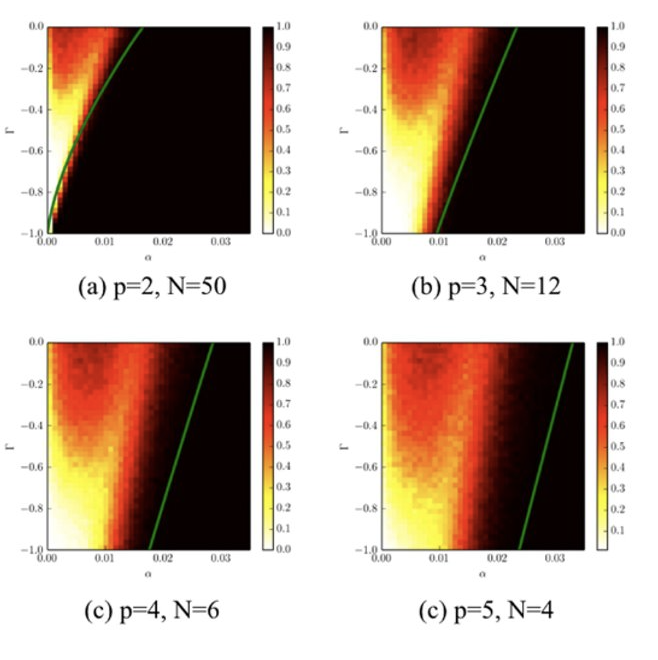
\includegraphics[width=0.6\textwidth]{Figures/GallaPrevalence}
    	\caption{ \label{fig::GallaPrevalence} Results as produced in
          the supplementary material of Sanders et al
          \cite{Sanders2018}. The same items appear here as in Figure
          \ref{fig::GallaPredictions}, except the value of p (number
          of players) increases moving from top left to bottom
          right. It is clear that the hotter region occupies a larger
          region of parameter space, indicating that as the bumber of
          players in the game increase, chaos becomes more prevalent.}
    \end{figure}

    Yet it can be argued that, for large populations of agents (e.g.,
    a crowd), the aggregate behaviour may be predictable, since the individual effect on the overall
    population is negligible \cite{Elamvazhuthi2019b}. This
    intuition is the foundation upon which crowd dynamics and flocking
    systems are based. In fact, the work presented by Leung et
    al. \cite{Hu2019} provides a cursory verification of this
    intuition. Here, the authors present an analysis of the learning
    dynamics for a large agent population (which they approximate as
    containing infinite agents) where each agent is an independent
    Q-Learning using Boltzmann action selection. The result is a
    system of equations, governed by a Fokker-Planck model which is
    numerically shown to be a strong predictor of the overall strategy
    selection of the population. Indeed, rather than examining the
    strategies of every agent in the population (which the authors
    approximate as infinitely large), they model the evolution of a
    probability density function which, for each action, defines the
    density of agents who retain a given Q-value for that action. This
    is illustrated in Figure \ref{fig::LeungPredictions}.

    \begin{figure}[h]
    	\centering
    	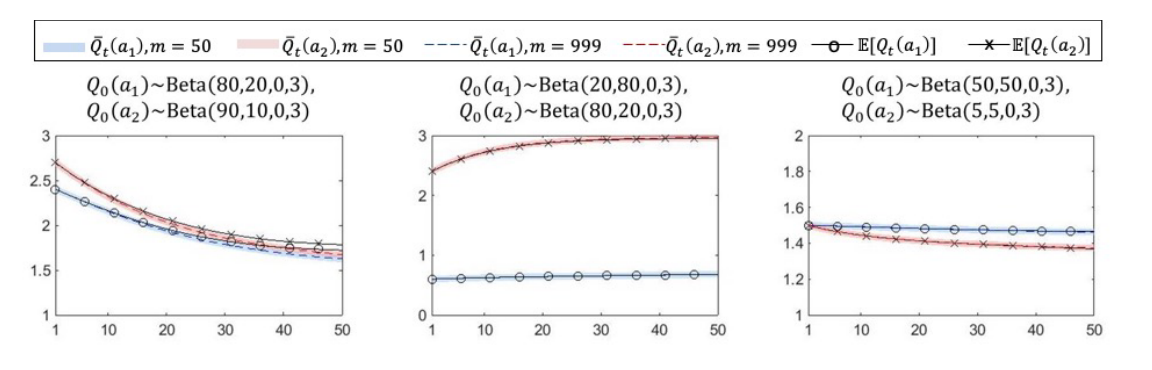
\includegraphics[width=0.9\textwidth]{Figures/LeungPredictions}
    	\caption{ \label{fig::LeungPredictions} Results as produced in Leung et al. \cite{Hu2019}.
    	Here, the solid and dotted lines represent the evolution of the expectation of Q-values of
    	two actions across a population of 50 or 999 agents respectively who are trained on an
    	iterated Stag Hunt game. The circled and crossed
    	lines represent the dynamics of these Q-values as predicted by the system of equations
    	derived in the paper. These are seen to closely match the results of the numerical
    	experiments.}
    \end{figure}

   	As the authors point out, this is the first attempt at considering such a problem, and relies on
	heavy assumptions. The strongest of these is placed on the game itself, which is always
	assumed to be cooperative (in Sanders' terms, $\Gamma = 1$). We, therefore, propose extending
	this model to accomodate an arbitrary choice of games. 

	The following are suggestions for approaching the estimation of large population dynamics.

	\begin{itemize}
		\item Estimate the population state through Random Finite Sets (RFS) and
	apply the models from the previous study. The aim here is to determine a state
	estimation for a swarm of unknown size through a random finite set by solving
	an optimal estimation problem  (typically iterated through a Kalman Filter
	\cite{Doerr2019}. As the swarm is treated probabilistically, the theory can
	accomodate an arbitrarily large system. Importantly, this may allow for the
	results from the previous section to be leveraged towards an arbitrary
	population. 

	\item Decompose a generic game into a weighted sum of a
	competitive and a cooperative game. Treat these as two separate agents and
	invoke the mean field approximation (MFA) so that any given agent is
	effectively engaged in a three-player game where the strategy of the opponents
	is the average strategy of the population. This leverages the existing results
	on the dynamics of three body problems in game theory \cite{Nagarajan2018} in
	a mixture of co-operative and competitive settings.
	\end{itemize}

	
	%\textbf{TODO: Elaborate on the technical details of the RFS and three body hypotheses}


    \section{Swarm Control through Fields} \label{sec::Swarm_Field_Control}

    Here we aim to study the interaction of a swarm of `active particles' with a potential field.
    In
    particular this field is to be generated by `field particles'. A Model Predictive Control 
    (MPC) scheme
    is to be devised to drive this system to desired configurations, with guarantees placed on
    stability and satisfaction of input constraints. The sub-optimality of the control
    scheme is to be studied.

    As described in Chapter \ref{ch::Lit_Review}, the control of swarms has been examined through the
    use of
    mean field models. These models resolve the fact that it is impossible to view the entire system
    as simply the sum of all of the agents and rather model the overall state of the system through
    density functions. Controls are then applied to this function whose evolution is described
    through, typically, one of two partial differential equations: the Fokker-Planck Equation (also
    referred to as the Kolmogorov Forward Equation) and the Vlasov Equation. The former has seen
    some success in recent literature \cite{Elamvazhuthi2019, Li2017,
    Roy2017}, though it makes the assumption that the system evolves through `drifted
    brownian motion'. This means that the agents are considered to move independently and
    randomly, though under the influence of a field which affects their velocity. This technique
	has been shown, both theoretically and experimentally, to drive swarm systems in a stable
	manner \cite{Fleig}. The latter is beginning to show promise 
	though control is typically through leadership rather than fields \cite{Burger2019}. 

	The hypothesis of this section is that the distribution of active particles, whose evolution is
	described through a Vlasov equation, may be controlled through the influence of a scalar field
	generated by `field paricles'. This is drawn from the dynamics posed by Bellomo et al. 
	\cite{Bellomo2017}

	\begin{equation}
	\label{eqn::Vlasov}
    \begin{split}    
        \partial_t f + \Vec{v} \cdot \nabla_{\Vec{x}} f + \kappa \nabla_{\Vec{v}} \cdot (F_a (f) f)
        = \epsilon Q(f, f) \quad  (\Vec{x}, \Vec{v}) \in \Omega[f] \times D_{\Vec{v}}, \quad t>0, \\
        F_a[f](t, \Vec{x}, \Vec{v}) = - \int_{\Omega [f] \times D_{\Vec{v}}} \psi (|\Vec{x} - \Vec
        {x^*}|)(\Vec{v} - \Vec{x^*}) f(t, \Vec{x}^*, \Vec{v}^*) d\Vec{x}^* d\Vec{v}^*, 
    \end{split}
    \end{equation}


    Here, $f = f(t, \Vec{x}, \Vec{v})$ is the one-particle probability density function at
    phase-space position ($\Vec{x}, \Vec{v}$), $\Vec{v}$ and time $t$ which represents the state of
    the system. $\kappa \geq 0$ is a scalar
    coefficient, $\psi$ denotes the communication strength between particles, and ($\Vec{x}^*, \Vec
    {v}^*$) gives the position in phase space of a `field particle'. It can be seen that the these
    field particles influence the velocity of the swarm agents.

	The contribution that this study presents over those using brownian motion is the inclusion of an
	interaction operator $Q(f, f)$. This governs how agents interact with one another. With this
	term included, the dynamics account for the tendency of agents to avoid collisions. However,
	the term is intended to account also for social interactions between agents, which we aim to
	leverage in the subsequent section.

	The complexity of this interaction term will need to be gradually increased over time. To begin
	with, we may entirely neglect this term. It is here that we will compare the model proposed by Zhang
	with that proposed by Bellomo et al. We may then consider only local interactions, which is typical
	for most swarming systems in the current literature, before then considering non-local interactions.
	This provides the scope for swarms to interact with a greater number of agents. At this stage, we
	may expand our study to consider the presence of interaction domains. This places constraints on how
	agents may interact with one another, allowing for a greater generalisation of inter-agent
	interactions. Ultimately, we would like to influence the interaction term, though this is discussed
	in Section \ref{sec::Intelligence_in_control}. The questions we will
	consider here are:

	\begin{itemize}
		\item The stablity of the system: Under what conditions is it possible to drive the
		swarm from one configuration to another in a stable manner? Fortunately, Bellomo et al.
		present a candidate lyapunov functional upon which dissipation can be evaluated, though it
		will need to be adapted for the consideration of the consensus models.
		\item The guarantees of the system: Is it possible to ensure that controls remain within an
		admissible set (typically a closed, bounded and convex set \cite{Fredi2010}).
		\item Whether the conservation laws of normalisation and total mass, as presented in 
		\cite{Bellomo2017} can be guaranteed.
	\end{itemize}

	These results will be established theoretically alongside the sub-optimality of the MPC scheme
	and verified through numerical simulations in a 2D environment. It
    will be of interest to perform a similar analysis to Ko and Zuazua \cite{Ko2019} in which the
    cost functional is altered to favour particular metrics  (e.g. running cost, control time etc.)
    and also analyse the effect of varying the time horizon.

    \section{Incorporation of Intelligence in Control} \label{sec::Intelligence_in_control}

    This section of the study is perhaps the strongest extension
    proposed in this chapter, and will likely be the most
    challenging. Here, we examine the dynamics (\ref{eqn::Vlasov}) in
    which the interaction term accounts for the social dynamics of the
    decision making of individual agents who have learnt through an
    iterated game. We leverage the strategy evolution dynamics and
    stability analysis established in \ref{ch::ShortTermGoals} and
    \ref{sec::Large_Agent_Dynamics}.

	Two proposals for incorporation of social interaction:
	\begin{itemize}
		\item Addition of the agent decisions as a constant in the state $f$. This will require that
		the decisions remain fixed in the state and so it will be required to make sure that the
		controls have no influence on this element.
		\item Weighted summation term in the probability of an agent changing its velocity from
		$v_*$ to
		$v$ due to a field particle with velocity $v^*$ $A[f](v_* \rightarrow v | v_*, v^*)$.
		Here, weights are equal to the agent strategy. This extends to both the swarms in
		which the leaders are making decisions (only leaders have this term) as well as in
		swarms where the population makes decisions (everyone has this term). This will need to be
		done with care though to ensure that normalisation holds. Note that, as this a probabilistic
		approach, we will need to examine the stochastic behaviour of the system and the extent to
		which constraint and conservation satisfaction can be guaranteed.
	\end{itemize}

	The MPC scheme from the previous section will then be adapted to this dynamical system with the
	same questions of well-posedness and stability considered. 

	A possible extension of this would be to consider online learning by incorporating the time
	evolution of the strategy space within the social interaction term, which would now be
	time-varying. The proper integration of these dynamical systems would depend on the form of the
	systems derived in Section \ref{sec::Large_Agent_Dynamics} and it is likely that relaxations would
	be required in terms of controllability results. An example would be to examine only the
	behaviour in the long-enough time frame, which means that we could not impose a final time. Of
	course, this means that we could only consider optimal control rather than model predictive.
	However, without establishing the models from Section \ref{sec::Large_Agent_Dynamics}, this
	extension is speculative and it is likely that such an extension would fall outside the scope of
	the PhD.

	%\textbf{TODO: elaborate on the technical details for proposals of social interaction, mention
	%the conservation laws}

\end{document}
